\section{Introduction}
\label{sec:introduction}

\subparagraph{Context.} 
\AP
A quasi-ordered set $(X, \leq)$ is \intro{well-quasi-ordered} (WQO)
if every non-empty subset of $X$ has a finite non-empty subset $Y \subfin X$ of
minimal elements, i.e. such that for every $x \in X$, there exists
$y \in Y$ such that $y \leq x$. When the set $X$ is totally ordered,
this is equivalent to the usual notion of well-ordering, but in the presence of 
incomparable elements, it is a stronger condition.
The theory of well-quasi-orderings (WQOs) is a powerful
combinatorial setting that has found applications in various areas of
mathematics and computer science. In graph theory, the celebrated result of
Robertson and Seymour~\cite{ROBSEY04} states that the class of all finite
graphs is well-quasi-ordered under the minor relation, a profound result with
deep algorithmic consequences. WQOs are also at the heart of
\emph{well-structured transition systems}, infinite state transitions systems
over which verification algorithms can be designed~\cite{ABDU96,ABDU98}. One of
the appeal of WQOs is that they are closed under various operations, such as
the sum and the product of WQOs. As an example, the closure of WQOs under the
finite words, also known as Higman's lemma \cite{HIG52}, has been used in the
verification of so-called \emph{lossy channel systems}~\cite{ABDU93}. 


% Well-quasi-ordered classes of graphs
\AP Undirected finite graphs are naturally equipped with the \reintro{induced
subgraph relation}, where $G$ is an induced subgraph of $H$ if $G$ can be
obtained from $H$ by deleting vertices (and the edges adjacent to them). Unlike
the graph minor relation, the induced subgraph relation is not a
well-quasi-ordering on the class of all finite graphs, as witnessed by the
infinite family of cycles of increasing size, which form an infinite antichain.
However, some classes of finite graphs are well-quasi-ordered under the induced
subgraph relation: for instance, the class of all finite paths, or the class of
all finite cliques. Distinguishing which classes of finite graphs are
well-quasi-ordered under the induced subgraph relation is a long-standing open
problem in graph theory, dating back to Pouzet's seminal work \cite{POUZ72}.

\AP In general, there is little hope to characterise all such classes, since
any countable order with finite infixes can be embedded into the induced
subgraph relation on finite graphs.\footnote{This is a folklore result.}
However, there are high hopes that a better notion of well-quasi-ordering on
classes of finite graphs is more amenable to structural characterisations. This
is why one usually considers \emph{labelled} well-quasi-orderings on classes of
finite graphs. Given a class $\Cls$ of finite graphs, and a well-quasi-ordering
$(X, \leq)$, one can consider the class $\Label{X}{\Cls}$ of graphs in $\Cls$
whose vertices are labelled by elements of $X$. The induced subgraph relation
is then extended to labelled graphs by requiring that the labels are preserved
by the embedding, i.e. that the label of a vertex in the smaller graph is less
than or equal to the label of its image in the larger graph. 

\begin{example}
  \label{ex:labelled-graphs}
  The class of all finite paths is not $2$-well-quasi-ordered,
  since the infinite sequence of paths with colored endpoints 
  forms an infinite antichain.
  The class of cliques is labelled-well-quasi-ordered,
  since any labelled clique can be identified with a multiset of labels,
  and the set of finite multisets over a WQO is itself WQO.
\end{example}


\AP
Bounded clique-width is a well-studied graph complexity measure
that generalises other well-known graph complexity measures such as
todo. There are several equivalent definitions of 
having \emph{bounded clique-width}, and we will use two 
of them in this paper. On the one hand, a class of graphs $\Cls$ has
\emph{bounded clique-width} if it is MSO-transducable from a class of finite
trees. On the other hand, a class of graphs $\Cls$ has 
\emph{bounded clique-width} if there exists a finite set of 
labels $\Sigma$ such that 
every graph in $\Cls$ can be constructed using the following operations:
\begin{itemize}
  \item creating a new vertex with label $a \in \Sigma$,
  \item taking the disjoint union of two labelled graphs,
  \item adding edges between all vertices of label $a$ and all vertices of label $b$,
  \item renaming all labels $a$ into $b$.
\end{itemize}

\begin{example}
  The class of all finite cliques, finite paths, finite cycles, 
  and finite trees all have bounded clique-width.
\end{example}

\begin{example}
  The class of all finite grids does not have bounded clique-width.
\end{example}



% ici mettre la figure de mon projet CNRS ?
% 
% -> exemples de classes + conjectures

\paragraph*{Contributions}
\AP
We prove that one can decide whether a class of graphs of bounded clique-width
is labelled-well-quasi-ordered, when the class is given by
an $\MSO$ interpretation from finite trees to undirected graphs.
Our proof scheme 




\paragraph*{Related works}

There are three natural conjectures that have been formulated 
regarding the relationship between various notions of well-quasi-ordering on
classes of finite graphs.

\begin{conjecture}[Pouzet \cite{POUZ72}]
    \label{pouzet:conj}
    Let $\Cls$ be a class of finite graphs.
    Then, the following are equivalent:
    \begin{enumerate}
      \item $\Cls$ is pointed-well-quasi-ordered,
      \item $\Cls$ is 2-well-quasi-ordered,
      \item $\Cls$ is labelled-well-quasi-ordered,
      \item $\Cls$ is wqo-well-quasi-ordered.
      \item $\Cls$ one can add a total order on the vertices of 
        its graphs, and remain wqo-well-quasi-ordered.
    \end{enumerate}
\end{conjecture}

\begin{conjecture}[{\cite[Conjecture 4]{DRT10}}]
  \label{thomasse:conj}
  Let $\Cls$ be a hereditary class of finite graphs of bounded clique-width.
  Then, $\Cls$ is $2$-well-quasi-ordered if and only if
  there exists $\Cls \subseteq \Cls[D]$ 
  ``structurally simpler'' such that $\Cls[D]$ is $2$-well-quasi-ordered.
\end{conjecture}


\begin{conjecture}[\cite{ALM17}]
  \label{lozin:conj}
  Let $\Cls$ be a hereditary class of finite graphs that is not labelled-well-quasi-ordered.
  Then, there exists 
  an infinite bad sequence of graphs in $\Cls$
  that is \emph{regular}.
\end{conjecture}

\begin{conjecture}[Schmitz's Transduction Conjecture]
    \label{transduction:conj}
    Let $\Cls$ be a class of finite graphs.
    Then, $\Cls$ is labelled-well-quasi-ordered
    if and only if
    $\Cls$
    does not existentially transduce all finite paths.
\end{conjecture}


\begin{conjecture}[Szymon's Collapsing Conjecture]
    \label{nip-cw:conj}
    Let $\Cls$ be a class of graphs.
    If $\Cls$ is labelled-wqo,
    then $\Cls$ is of bounded clique-width.
\end{conjecture}

\begin{figure}
    \centering
    \begin{tikzpicture}[
        conj/.style={rounded corners, thick, dashed, 
            A4
        },
        impl/.style={->, double},
        constr/.style={rounded corners,minimum width=1.7cm,minimum height=1cm,draw,rectangle,align=center}]
        \node[constr] (1w) at (0,0) {One \\ label};
        \node[constr] (2w) at (2,0) {Two \\ labels};
        \node[constr] (kw) at (4,0) {$k < \infty$ \\ labels};
        \node[constr] (lw) at (6,0) {Finite set \\ of labels};
        \node[constr] (ww) at (8,0) {WQO set    \\ of labels};

        \draw[conj]
        ($(lw.south west) + (-0.1, -1.1)$) rectangle ($(ww.north east) + (0.1, 0.1)$);

        \draw[conj]
        ($(2w.north west) + (-0.1, 1.1)$) rectangle ($(lw.south east) + (0.1, -0.1)$);
        \coordinate (P1m) at ($(2w.north)!0.5!(lw.north)$);
        \coordinate (P2m) at ($(lw.south)!0.5!(ww.south)$);
        \node (P1) at ($(P1m) + (0, 0.7)$) {\cref{pouzet1:conj}};
        \node (P2) at ($(P2m) + (0, -0.7)$) {\cref{pouzet2:conj}};

    \end{tikzpicture}
    \caption{The four well-quasi-ordering properties one can consider
             on classes of finite graphs.}
    \label{graph-properties:fig}
\end{figure}



\subparagraph*{Proof Techniques and Overview.} The overall proof technique can be
summarised in \cref{fig:proof-technique}. Given a class $\Cls$ of graphs
defined as the image of an $\MSO$ interpretation $I$ from finite trees to
graphs, we want to decide whether $\Cls$ is labelled-well-quasi-ordered. To
this end, we will use the following folklore result: if $(X, \leq)$ is a WQO,
and $f \colon X \to Y$ is a surjective order-preserving map, then $(Y, \leq)$
is also WQO. Because there exists a good candidate for $X$, namely, the set of
trees with Kruskal's tree embedding relation, we will try to see whether $I$ is
order-preserving. It turns out that for general interpretations, this is not
true (see \cref{example:msotree-not-monotone}). However, leveraging tools from
automata theory in the name of \emph{ramseyan factorisations} \cite{COLC07}, we
will be able to ``massage'' the input trees using a function $F$ into
\emph{nested trees}, with the property that for a good notion of ordering on
nested trees (nested Kruskal embedding essentially), the function $J$ that
factors $I$ through $F$ is order-preserving if and only if $\Cls$ is
labelled-well-quasi-ordered.

This proof technique will actually allow us to derive stronger results since it
shows that embeddings on graphs in $\Cls$ can be assumed to respect a certain
tree-like structure, and a fortiori, a linear order on the vertices of the
graphs. This will allow us to show that \cref{pouzet:conj} holds for classes of
graphs of bounded clique-width. Furthermore, listing the obstructions for $J$
to be order-preserving will allow us to show that counter-examples are regular
in nature, yielding a proof of \cref{lozin:conj} for classes of graphs of
bounded clique-width. Finally, the tree-like structure obtained is a form of
simple tree decomposition, answering positively to \cref{thomasse:conj} in
totality.

\begin{figure}
  \centering
  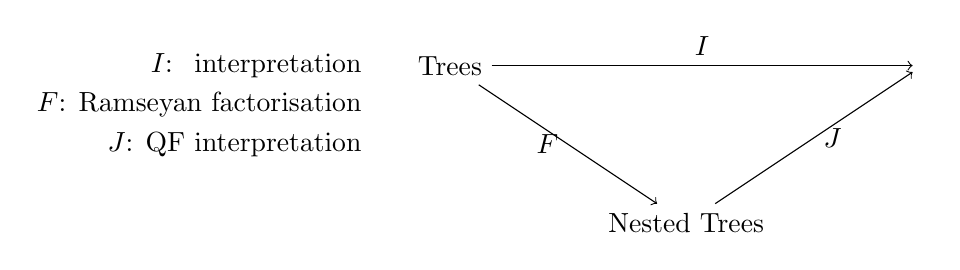
\begin{tikzpicture}
    \node (trees) at (0,0) {Trees};
    \node (graphs) at (6,0) {$\Cls$};
    \node (nested) at (3,-2) {Nested Trees};

    \draw[->] (trees) to node[above] {$I$} (graphs);
    \draw[->] (trees) to node[left] {$F$} (nested);
    \draw[->] (nested) to node[right] {$J$} (graphs);

    \node[anchor=east] (labelI) at (-1,0) {$I$: $\MSO$ interpretation};
    \node[anchor=east] (labelF) at (-1,-0.5) {$F$: Ramseyan factorisation};
    \node[anchor=east] (labelJ) at (-1,-1) {$J$: QF interpretation};
  \end{tikzpicture}
  \caption{Overview of the proof technique.}
  \label{fig:proof-technique}
\end{figure}


\paragraph*{Outline}



This explains the \emph{bottom-up} research direction in the field of WQOs,
which is to understand which \emph{constructors} preserve the WQO property:
finite sums, finite products, finite words, finite trees, finite graphs
\emph{with the minor relation} etc. It is motivated by the idea that one can
build complex orderings to model a concrete system by combining simpler ones,
and has empirically shown to be a fruitful approach (see \cite{HSS13} for an
example of nesting Higman's orderings). One other research direction is to
devise \emph{decision procedures} that take as input a set and decide whether
it is WQO or not, and whether classical decision algorithm on well-structured
transition systems can be applied to the concrete model one has. This dual
\emph{top-down} approach also had its recent share of successes
\cite{ALM17,FINGU19,LOPEZ24}.




\subparagraph{A Model-Theoretic Approach to WQOs.}
\AP 
While finite products and sums are natural algebraic constructions on sets, the
cornerstone results of Higman and Kruskal showing that well-quasi-ordered sets
are closed under \emph{finite words} \cite{HIG52} and \emph{finite trees}
\cite{KRU72} require a careful definition of the ordering on those structures,
together with a non-trivial and tailored proof that they are
well-quasi-ordered, often requiring the use of a so-called \emph{minimal bad
sequence argument} \cite{NASH65}. We argue that the better way to introduce
these orderings stems from a model-theoretic approach to WQOs, where one
considers subsets of \emph{finite structures} endowed with the usual notion of
\emph{embedding} (of models). Considering finite words as labelled total orders
one immediately sees that the seemingly \emph{ad-hoc} definition of the
\emph{subword ordering} powering Higman's lemma is in fact an instance of the
usual embedding relation from logic. A similar observation can be made for
Kruskal's tree theorem, where structures are labelled trees equipped with the
least common ancestor relation. These are folklore results, but we believe that
they are a strong motivation for a more systematic study of the embedding
relation on classes of finite structures.

\AP In this context, the simplest (non-trivial) structures one can consider are
\emph{finite undirected graphs}. The corresponding notion of embedding is the
\emph{induced subgraph relation} that is well-known from graph theory. Given a
class $\Cls$ of finite undirected graphs, one can as whether $\Cls$ is
well-quasi-ordered under the induced subgraph relation. One can also consider
$\Cls$ as a \emph{constructor} for new WQOs, mapping $(X, \leq)$ to
$\Label{X}{\Cls}$, the class of graphs in $\Cls$ labelled using elements of
$X$, this is how one obtains $X^*$ from $X$ in Higman's lemma. The natural
question is then, whether $\Label{X}{\Cls}$ is WQO when $X$ itself is WQO.
Freely labeling classes of graph is an operation that is prominent in the field
of \emph{structural graph theory}: this is for instance the difference between
being NIP and being \emph{monadically} NIP \todo{cite}. However, in this
context,  the set $X$ of labels is equipped with the equality relation and is
finite. Of course, one can also consider further restrictions on $X$, such as
requiring that $X$ is of size at most $k$ for some $k \in \Nat$. We  depicted
in
\cref{graph-properties:fig},
these various properties, and the two conjectures of Pouzet claiming that these
potentially distinct notions all collapse to either being \kl{WQO} or
\kl{wqo-WQO}. We state the two conjectures separately because only the first
one is explicitly found in \cite{POUZ72}.

In general, the class of all finite graphs (even undirected and unlabelled) is
not well-quasi-ordered under the induced subgraph relation (for instance, the
class of finite cycles forms an infinite antichain).

There have been many attempts to understand
which classes of (finite) graphs are WQOs when endowed with the induced
subgraph relation. One can think of the early work of Ding on classes of
bounded tree-depth \cite{DING92}, or more recent approaches
\cite{DRT10,DLP17,POZA22}.
Typical proofs that a set is well-quasi-ordered can be clustered into two
categories: \emph{structural proofs} that exhibit an encoding of the set into a
well-quasi-ordered set built from simpler elements, and \emph{minimal bad
sequence arguments} \cite{NASH65}. The latter are often tedious and error-prone
to carry out \cite[Discussion xxx]{LOPEZ23}. 

Attempts to prove these conjectures often relied on assuming some kind of
structural property of the class of graphs, such as enjoying suitable
\emph{tree decompositions}.

Now, to work on those trees, one needs to place a well-quasi-ordered relation
on them. This is usually done using the tree embedding relation, also known as
Kruskal's embedding relation, which is a well-quasi-ordering on trees
\cite{KRU72}. This works when the function that maps a tree to a graph is
simple enough, but more often than not, this is not the case. In \cite{DRT10},
the authors introduce a \emph{tailored} embedding relation on trees, and prove
that it is a well-quasi-ordering under certain hypotheses, leveraging a tedious
and error-prone proof using a \emph{minimal bad sequence argument}
\cite{NASH65}. \todo{talk about clique width now}

We know since \cite{FREU20} and \cite{LOPEZ23} that one can easily inductively
define well-quasi-orderings of increasing complexity on a given set. One
example of such a construction is the \emph{gap embedding relation} of
Derhowitz and Tzameret \cite{DERSHOWITZ200380}. This relation was already at
the core of \emph{priority channel systems}, although in a somewhat hidden form
\cite{HSS13}.  It was also noticed in \cite{LOPEZ24} that the \emph{ad-hoc}
construction of \cite{DRT10} was in fact a particular instance of the gap
embedding relation on trees.

A line of research initiated in \cite{LOPEZ24} explores the \emph{automata
theoretic} approach to the Pouzet conjectures. It was conjectured that the
notion of gap-embedding could be useful. We prove that this is the case.
\todo{Relied on monoids and automata theory on words}
\textbf{The gap embedding is essentially the only well-quasi-ordering on 
graph that can exist.}


Recently, a conjecture was formulated by Sylvain Schmitz in a personal
communication with the authors, which we will call the \emph{transduction
conjecture}. It attemps to bridge the gap between the study of
\kl{well-quasi-ordered} classes of graphs that are ``combinatorially
well-behaved'' and the field of ``structural graph theory'' that focuses on
class that are ``first-order well-behaved''.




The motto would then be ``the only well-quasi-orderings on graphs are the gap
embeddings'' and would provide a fundamental barrier to the complexity of
induced subgraph well-quasi-orderings.

\clearpage

\paragraph*{Contributions.}

At the core of our analysis is the fundamental connection between a deep
automata theoretic construction (the existence of \emph{forward ramseyan
factorisations} on trees \cite{COLC07}) and a deep combinatorial construction
(\emph{gap embedding} on trees \cite{DERSHOWITZ200380}). These two
constructions were meant to be used together, as we will try to advocate in
this paper. This allows us to prove the following result:

\begin{theorem}
  Let $\Cls$ be a class of graphs having \kl{bounded clique-width}.
  The following are equivalent:
  \begin{enumerate}
    \item $\Cls$ is \kl{wqo-well-quasi-ordered}
    \item For every class $\Cls[D] \subseteq \Cls$ of graphs of \kl{bounded linear clique-width},
      $\Cls[D]$ is \kl{wqo-well-quasi-ordered}
  \end{enumerate}
  Furthermore, this properties are decidable when $\Cls$ is given 
  by an $\MSO$ interpretation from finite trees to undirected graphs.
\end{theorem}

By carefully analysing the proof of \cite{LOPEZ24}, we are able to reformulate
their main result in terms of \kl{bounded one-dimensional-linear-clique-width},
a very strong restriction on the class of graphs, which is defined below.

\begin{definition}
  A class of graphs $\Cls$ has \intro{bounded one-dimensional-linear-clique-width}
  if there exists a word $w \in \Sigma^*$, where $\Sigma$ is a finite alphabet,
  and an $\MSO$ interpretation $\phi$ from finite words to undirected graphs
  such that $\Cls \subseteq \phi(w^*)$.
\end{definition}

\begin{theorem}
  Let $\Cls$ be a class of graphs having \kl{bounded linear-clique-width}.
  The following are equivalent:
  \begin{enumerate}
    \item $\Cls$ is \kl{wqo-well-quasi-ordered}
    \item For every class $\Cls[D] \subseteq \Cls$ of graphs of
      \kl{bounded one-dimensional-linear-clique-width},
      $\Cls[D]$ is \kl{wqo-well-quasi-ordered}
  \end{enumerate}
  Furthermore, this properties are decidable when $\Cls$ is given 
  by an $\MSO$ interpretation from finite trees to undirected graphs.
\end{theorem}

On these very restricted classes, it becomes easy to witness the truth of all
the Pouzet conjectures, and as well as the Schmitz transduction conjecture in a
weak from.

\begin{theorem}
  Let $G$ be an idempotent graph,
  and $\Cls \defined \setof{ G^n }{n \in \Nat}$.
  Then, the following are equivalent:
  \begin{enumerate}
    \item $\Cls$ is \kl{wqo-well-quasi-ordered}
    \item $\Cls$ is \kl{labelled-well-quasi-ordered}
    \item $\Cls$ is \kl{2-well-quasi-ordered}
    \item $\Cls$ is \kl{pointed-well-quasi-ordered}
    \item $\Cls$ does not existentially transduce
      graphs of arbitrarily large diameter.
  \end{enumerate}
\end{theorem}

As a consequence of these results,
we obtain 

\begin{theorem}
  Let $\Cls$ be a \emph{hereditary} class of \kl{bounded clique-width}.
  Then, the following are equivalent:
  \begin{enumerate}
    \item $\Cls$ is \kl{wqo-well-quasi-ordered}
    \item $\Cls$ is \kl{pointed-well-quasi-ordered}
    \item $\Cls$ does not existentially transduce
      the class of all finite paths.
  \end{enumerate}
  Furthermore, this properties are decidable when $\Cls$ is given
  by an $\MSO$ interpretation from finite trees to undirected graphs.
\end{theorem}

\paragraph*{Outline.}
